\begin{minipage}{0.48\linewidth}
	On décide de simuler un FAR(1) basé sur un opérateur linéaire intégral :

	\begin{equation*}
		X_{n+1} = \phi(X_n) + \varepsilon_{n+1}
	\end{equation*}

	avec : $\phi : f \mapsto \displaystyle\int_{\mathcal T} f(u) \beta(u, \cdot \,) \, du$

	C'est une modélisation fréquente des FAR(1). Le noyaux que l'on considère dans l'opérateur intégral pour les simulations est le suivant :


	\begin{equation*}
		\beta : \, \begin{array}{ccc}
			[0,1]^2 & \longrightarrow & \mathbb R
			\\
			(t,s)   & \longmapsto     & \frac 9 4 t\sqrt{ s(1-s) }
		\end{array}
	\end{equation*}

\end{minipage}
\hfill
\begin{minipage}{0.48\linewidth}
	\begin{figure}[H]
		\centering
		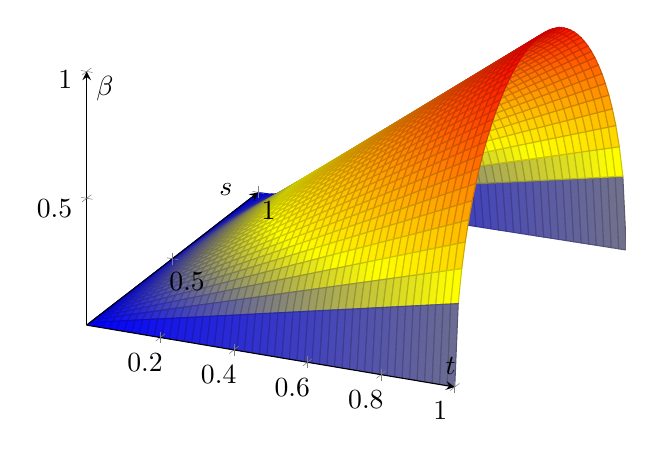
\begin{tikzpicture}
			\begin{axis}[
					xlabel=$t$,
					ylabel=$s$,
					zlabel=$\beta$,
					xmin=0, xmax=1,
					ymin=0, ymax=1,
					zmin=0, zmax=1,
					axis lines=center,
					axis on top=true,
					domain=0:1,
					samples=50,
				]
				\addplot3 [surf] {9/4*x*sqrt(y*(1-y))};
			\end{axis}
		\end{tikzpicture}
		\caption{Graphique du noyau intégral pour la relation FAR(1)}
		\label{graph:far_kernel}
	\end{figure}
\end{minipage}

\bigskip

On notera que le noyaux utilisé pour la relation de $\operatorname{FAR}(1)$ est une fonction lisse. Ainsi il remplit aisément la condition pour que le $\operatorname{FAR}(1)$ hérite de la régularité du mouvement brownien multi-fractionnaire généré.
